\documentclass[12pt,a4paper]{article}
\usepackage{indentfirst,latexsym,graphicx}
\usepackage[utf8]{inputenc} % Включаем поддержку UTF8
\usepackage[russian]{babel}
\usepackage{amssymb,amsmath}
\graphicspath{{img/}} % тут картинки твои
\usepackage[left=2cm,right=2cm,top=2cm,bottom=2cm,bindingoffset=0cm]{geometry}
\usepackage{amsmath, amssymb, amsthm}

\begin{document}
Принципиальная схема:
\begin{center}
        \begin{figure}[h!]
                \center{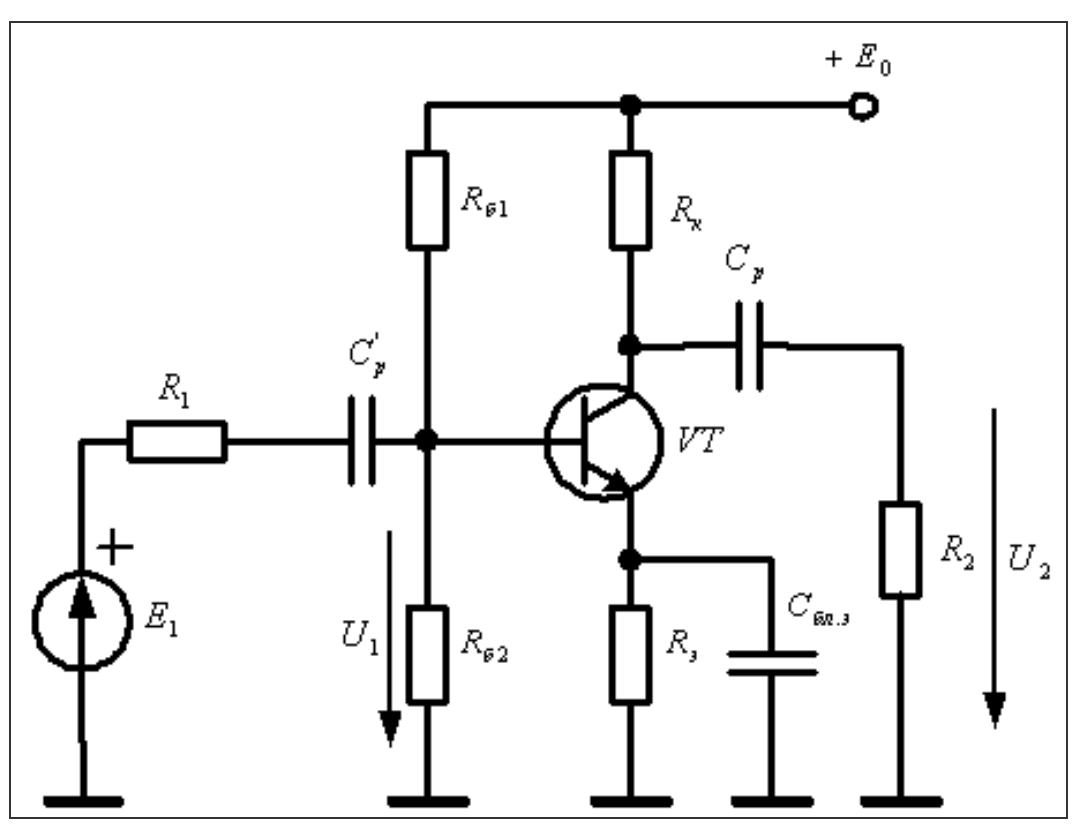
\includegraphics[scale=0.2]{oe.png}}
                \caption{Могут ли каскады ОЭ, ОБ,ОК иметь одинаковые большую верхнюю граничную частоту}
        \end{figure}
\end{center}

берем из 11 вопроса все, кроме того, что касается ОК. Из табл видно, что совпадают

\end{document}
